\subsection{ソフトウェア設計品質分析と評価}

設計は、作ったら終わりではない。設計が要求を満たすか、品質属性を達成できるか、保守しやすいか、リスクが残っていないかを分析・評価する必要がある。

\subsubsection{設計レビューと監査}

\term{設計レビュー}{Design Review} は、設計を包括的に調べる活動である。目的は、設計の完成度、要求の網羅、未解決事項、潜在問題、品質リスクを確認することである。レビューは、設計チーム自身、独立した第三者、顧客、品質保証担当などによって行われる。

\term{設計監査}{Design Audit} は、より狭い観点に焦点を当てる。たとえば、特定の機能監査、標準への適合監査、セキュリティ方針への適合監査などである。

\par\smallskip
\begin{center}
\centering
\IfFileExists{assets/generated_figures/ch03/fig-ch03-11.png}{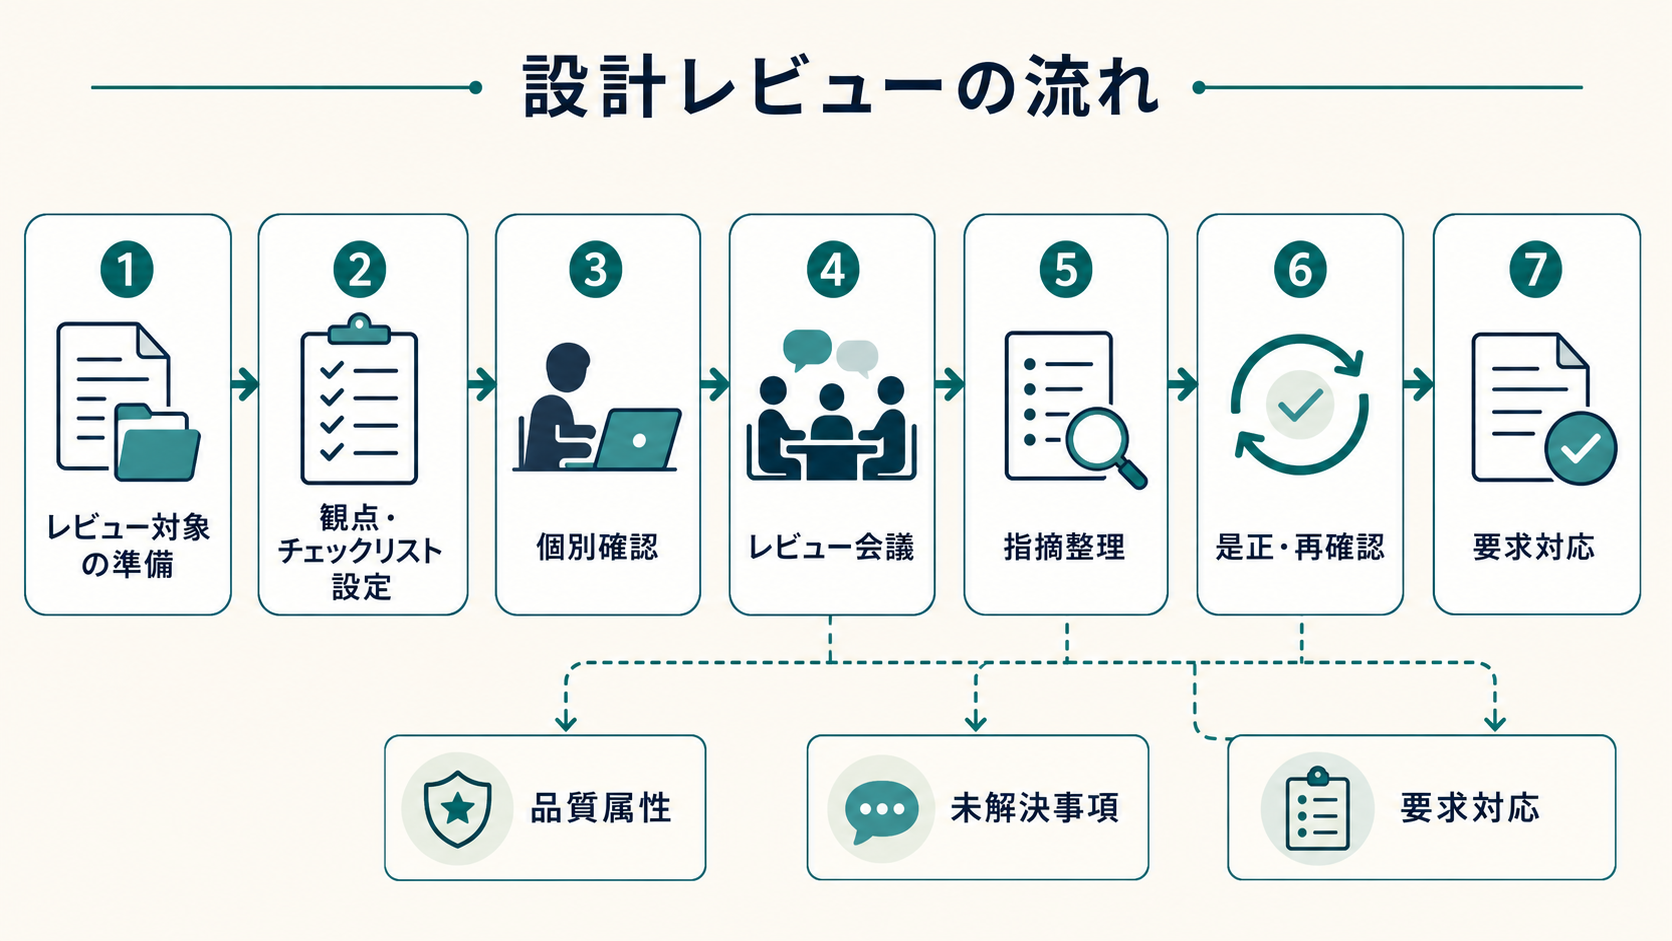
\includegraphics[width=0.96\linewidth]{assets/generated_figures/ch03/fig-ch03-11.png}}{\fbox{\parbox[c][48mm][c]{0.9\linewidth}{\centering 画像生成待ち\\設計レビューの流れ}}}
\par\smallskip
\refstepcounter{figure}\label{fig:ch03-11}図 \thefigure: 設計レビューの流れ
\end{center}
図 \thefigure は、設計レビューの流れを視覚的に整理したものである。
\par\smallskip

\subsubsection{品質属性}

設計品質に関わる属性には、モジュール性、保守容易性、移植性、テスト容易性、使いやすさ、正しさ、堅ろう性などがある。これらは、利害関係者の関心事の大きな部分を占める。

品質属性には、実行時に観察できるものと、実行時には直接見えにくいものがある。性能、セキュリティ、可用性、機能性、使いやすさは、実行時に観察しやすい。一方、変更容易性、移植性、再利用性、テスト容易性は、設計や保守の中で評価されることが多い。概念的一貫性、正しさ、完全性は、設計記述そのものを見て評価される。

\subsubsection{品質分析・評価技法}

設計品質を分析・評価するための技法には、静的分析、シミュレーション、プロトタイピング、レビュー、要求追跡などがある。

\par\smallskip\noindent\refstepcounter{table}\label{tab:ch03-06}表 \thetable: 品質分析・評価技法の整理\par\smallskip
表 \thetable は、品質分析・評価技法の整理を比較・確認しやすい形で整理したものである。\par\smallskip
\begin{tabularx}{\linewidth}{L{36mm}Y}
\toprule
技法 & 説明 \\
\midrule
設計レビュー・検査 & 設計記述を人が確認し、要求対応、未解決事項、設計上のリスクを見つける。 \\
シナリオに基づく評価 & 利用シナリオ、障害シナリオ、変更シナリオを使って、設計がどう反応するか確認する。 \\
要求追跡 & 要求が設計要素へ対応しているか、設計要素に根拠となる要求があるか確認する。 \\
静的分析 & 実行せずに設計やモデルを分析する。依存関係、循環、整合性、弱点を確認する。 \\
形式的分析 & 数学的モデルを使い、性質を厳密に検査する。安全性やセキュリティが重要な領域で有効である。 \\
シミュレーション & 設計モデルを使い、性能、タイミング、負荷、失敗時の挙動などを試す。 \\
\term{プロトタイピング}{Prototyping} & 実現可能性、使いやすさ、技術的リスクを確認するために試作品を作る。 \\
\bottomrule
\end{tabularx}

\par\smallskip
\begin{center}
\centering
\IfFileExists{assets/generated_figures/ch03/fig-ch03-12.png}{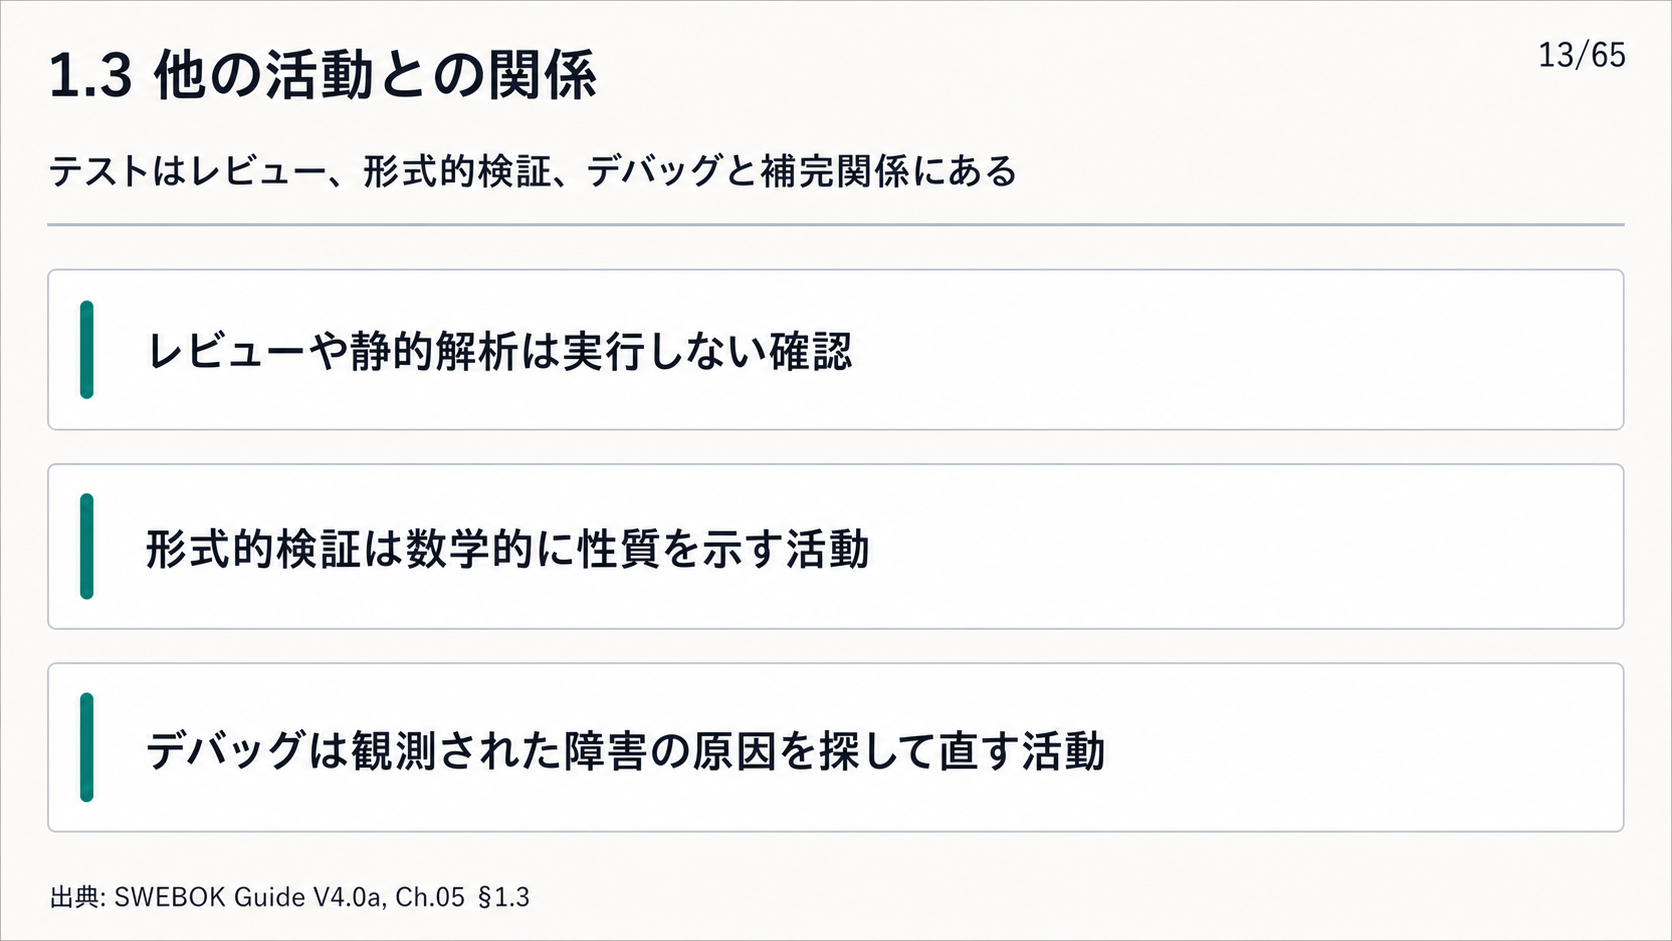
\includegraphics[width=0.96\linewidth]{assets/generated_figures/ch03/fig-ch03-12.png}}{\fbox{\parbox[c][48mm][c]{0.9\linewidth}{\centering 画像生成待ち\\品質分析・評価技法の比較図}}}
\par\smallskip
\refstepcounter{figure}\label{fig:ch03-12}図 \thefigure: 品質分析・評価技法の比較図
\end{center}
図 \thefigure は、品質分析・評価技法の比較図を視覚的に整理したものである。
\par\smallskip

\subsubsection{測度とメトリクス}

\term{測度}{Measure} と\term{メトリクス}{Metric} は、設計の大きさ、構造、複雑さ、品質を定量的に見るために使われる。測定対象は、設計方法によって異なる。

機能分解を中心とする設計では、構造チャートなどから、階層の深さ、モジュール数、呼び出し関係の複雑さを測る。オブジェクト指向設計では、クラス図などから、クラス数、継承の深さ、結合度、凝集度、メソッド数、メッセージ数などを測る。

測度は、設計の良し悪しを自動的に決めるものではない。測度は、注意すべき箇所を見つける手がかりである。たとえば、結合度が高い部品は変更の影響が大きい可能性がある。凝集度が低い部品は責務が散らばっている可能性がある。

\subsubsection{検証・妥当性確認・認証}

設計の分析と評価は、検証、妥当性確認、認証に関わる。

\par\smallskip\noindent\refstepcounter{table}\label{tab:ch03-07}表 \thetable: 検証・妥当性確認・認証の整理\par\smallskip
表 \thetable は、検証・妥当性確認・認証の整理を比較・確認しやすい形で整理したものである。\par\smallskip
\begin{tabularx}{\linewidth}{L{32mm}Y}
\toprule
活動 & 意味 \\
\midrule
\term{検証}{Verification} & 設計が、明示された要求を満たしているかを確認することである。 \\
妥当性確認 & その設計で作られるシステムが、顧客、利用者、運用者、保守担当者の期待を満たせるかを確認することである。 \\
\term{認証}{Authentication} & 第三者が、設計が仕様や意図された利用に適合していると証明または表明することである。 \\
\bottomrule
\end{tabularx}

検証は「要求どおりか」を問う。妥当性確認は「本当に役に立つか」を問う。認証は「決められた基準に適合していると第三者が認めるか」を問う。安全性や規制が重要な領域では、設計段階から認証を見据えた証拠を残す必要がある。
